\documentclass{article}
\usepackage{tikz}
\usetikzlibrary{calc}
\begin{document}
% for循环与let语句

\begin{tikzpicture}
    % for循环参考section 88,第1001页
    % for循环应用于单个语句: 
    % \foreach \<var_name> [<options>] in {<list>} 
    %   <cmd>;
    % list格式:
    %   1.<num_1>,<num_2>,<num_3>  完整列出列表
    %   2.<num_1>,<num_2>,...,<num_n>  以num_2-num_1为步进, 补足列表中间的数
    %   3.<num_1>,...,<num_n>  以步进为1(num_n > num_1)或-1(num_n < num_1)
    \foreach \x in {1,2,...,5} 
      \draw (\x,0) circle [radius=2pt];

    % for循环应用于多个语句:
    % \foreach \<var_name> [<options>] in {<list>} 
    %   {<cmd>}
    \foreach \x in {1,2,...,5}
      {
        \draw (\x,0) circle [radius=2pt];
        \fill (\x,0) circle [radius=1pt];
      }
\end{tikzpicture}\\\vspace{1cm}

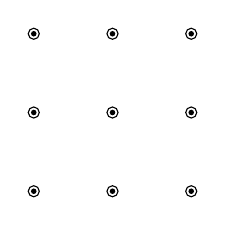
\begin{tikzpicture}
    % 多层foreach嵌套
    \foreach \x in {0,1,2}
      \foreach \y in {0,1,2}
        {
          \draw (\x,\y) circle [radius=2pt];
          \fill (\x,\y) circle [radius=1pt];
        }
\end{tikzpicture}\\\vspace{1cm}

\begin{tikzpicture}
    % 迭代item为坐标点
    \foreach \x in {(1,1),(2,2),(5,5)}
      {
        \draw \x circle [radius=2pt];
        \fill \x circle [radius=1pt];
      }
\end{tikzpicture}\\\vspace{1cm}

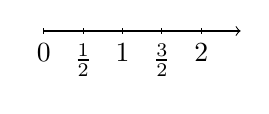
\begin{tikzpicture}
    % for循环的多个变量
    % \foreach \<var_01>/\<var_02> in {<num_01_1>/<num_02_1>,<num_01_2>/<num_02_2>,<num_01_3>}
    % 多个变量名称使用/分隔, 每一组变量值中, 使用/分隔分配给不同变量的值; 如果组内后续变量值没有赋予, 则沿用前面变量的值(如num_02_3 = num_01_3)
    \draw[->] (0,0) -- (2.5,0);
    \foreach \x/\y in {0,0.5/\frac{1}{2}, 1, 1.5/\frac{3}{2},2}
      {
        \draw (\x,-1pt) node[below]{$\y$} -- (\x,1pt);
      }
\end{tikzpicture}\\\vspace{1cm}

\begin{tikzpicture}
    %   for循环的list item默认不进行数学计算,evaluate对list item进行数学计算
    \foreach \x in {2^0,2^...,2^9}
      $\x$;

    % foreach的可选参数
    % 1.evaluate
    %   (1)evaluate=<variable>
    %     将计算评估结果覆盖到原变量
    \foreach \x [evaluate=\x] in {2^0,2^...,2^9}
      $\x$;

    %   (2)evaluate=<variable> as <other_variable>
    %     将计算评估结果放到其他变量
    \foreach \x [evaluate=\x as \y] in {2^0,2^...,2^9}
      $\y$;

    %   (3)evaluate=<variable> as <other_variable> using <formula>
    \foreach \x [evaluate=\x as \y using 10*\x] in {2^0,2^...,2^9}
      $\y,\,$;
\end{tikzpicture}\\\vspace{1cm}

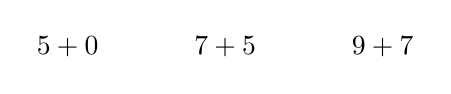
\begin{tikzpicture}
    % foreach的可选参数
    % 2.remember=<variable> as <macro> (initially <value>)
    %   将当前循环的变量值,保留到特殊变量,可以在下一次循环使用,并且可以使用initially赋予特殊变量一个初始值(默认为0)
    \foreach \x [remember=\x as \xsave] in {5,7,9}
      \node at (\x,0){$\x+\xsave$};
\end{tikzpicture}\\\vspace{1cm}

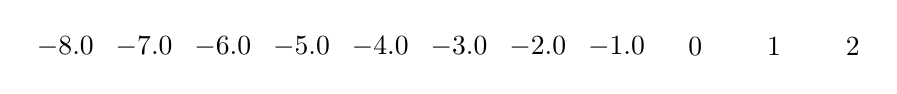
\begin{tikzpicture}
    % foreach的可选参数
    % 3.parse=true
    %   将list item的内容给\pgfmathresult进行计算,常配合evaluate参数一起使用
    \def\mvalue{2}
    \foreach \x [parse=true,evaluate=\x] in {\mvalue-10,...,\mvalue}
      \node at (\x,0){$\x$};
\end{tikzpicture}\\\vspace{1cm}

% \breakforeach, 不管该指令在其他语句之前或之后,都会执行完当前循环才跳出循环,所以效果等同于放在所有语句的最后

\begin{tikzpicture}
    % \path let <assign_state> in <statement>;
    % 在assign_state中对变量进行赋值,多个赋值使用','分隔,需要使用calc库. 变量类型列表: 
    %     \p{<registor_name>}=<coordinate> - 坐标点,未指定长度单位时,默认为pt;指定其他长度单位时,底层转化为pt单位对应长度
    %     \x{<registor_name>}=<val>|<dimension> - 坐标点的x值,未指定长度单位时,默认为pt;指定其他长度单位时,底层转化为pt单位对应长度
    %     \y{<registor_name>}=<val>|<dimension> - 坐标点的y值,未指定长度单位时,默认为pt;指定其他长度单位时,底层转化为pt单位对应长度
    %     \n{<registor_name>}={<formula>} - 代表纯数字,或长度值(底层转化为pt). 只要公式中携带长度单位,则n为长度值
    \draw[->] (-4,0) -- (4,0) node[right]{$x$};
    \draw[->] (0,-4) -- (0,4) node[above]{$y$};
    \draw (-3,-3) grid[step=1cm] (3,3);
    \draw
      let
        \p1  = (1,1),
	\p2  = (3,3)
      in
        (\p1) circle [radius=2pt]
	(\p2) circle [radius=2pt]
	(\x1,\y2) circle [radius=2pt];
\end{tikzpicture}\\\vspace{1cm}

\begin{tikzpicture}
    % let命令,以指定长度为圆半径
    \coordinate (A) at (1,0);
    \coordinate (B) at (4,4);
    \filldraw (A) circle [radius=1.2pt];
    \filldraw (B) circle [radius=1.2pt];
    \draw
      let
        \p1=($(B)-(A)$),
        \n1={veclen(\x1,\y1)}
      in
        (A) circle [radius=\n1];
\end{tikzpicture}

\begin{tikzpicture}
    % \pgfextra{\pgfmathsetmacro{\mylen}{\n}}将长度值提取非单位数值
    \path[draw,name path=circle] (0,0) circle [radius=2];
    \filldraw (0,0) circle [radius=1.2pt];
    \node[left] at (0,0){$O$};
    \path 
      let 
        \p1 = (0,0),\p2 = (4,0),
        \n1 = {2cm},\n2 = {veclen(\x2-\x1,\y2-\y1)},
        \n3 = {asin(\n1/\n2)}
      in  
        \pgfextra{\pgfmathsetmacro{\mylen}{\n3}}
        [draw,name path=AB,rotate around={-\mylen:(\p2)}] (\p2) -- (\p1);
\end{tikzpicture}
\end{document}
